\chapter{RL Distribuido}%
\label{cha:rl_distribuido}

\lecture{17}{2020-07-13}{Distributed RL}

\section{Patrones computacionales comunes en RL}%
\label{sec:patrones_computacionales_comunes_en_rl}

Se han visto algoritmos que actualizan la política a partir de un batch de observaciones. Esto
se hace en contraposición de los algoritmos online ya que de esta forma se está aprovechando
todo el poder computacional de las CPU de forma paralela.

\begin{center}
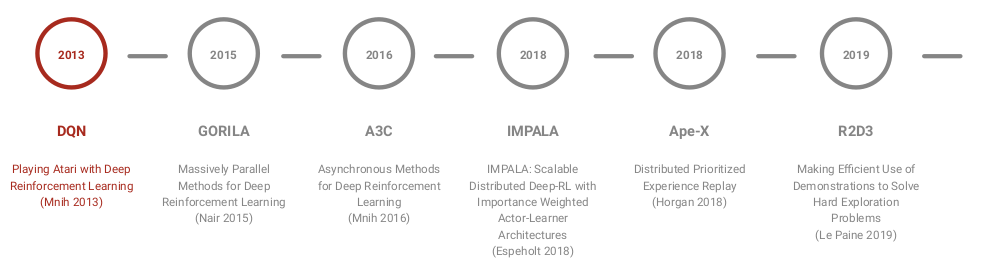
\includegraphics[width=0.8\textwidth]{figures/2020-07-13-141912_981x267_scrot.png}
\end{center}

\begin{itemize}
    \item DQN (2013-2015): no es distribuido ni paralelizado pero introduce ideas que serán
        útiles para ello.
    \begin{center}
        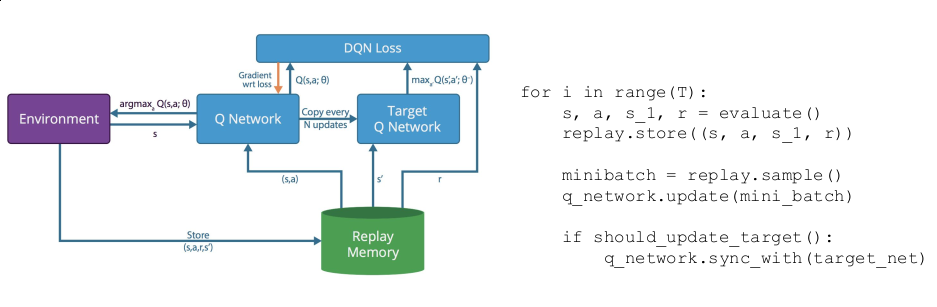
\includegraphics[width=0.8\textwidth]{figures/2020-07-13-142101_937x307_scrot.png}
    \end{center}
    Se tiene un agente que evalúa un entorno y los datos recogidos se guardan en un buffer. De
    este buffer se recogen batches aleatorios que sirven para actualizar las redes
    neuronales.
    \item GORILA (2015): 
    \begin{center}
    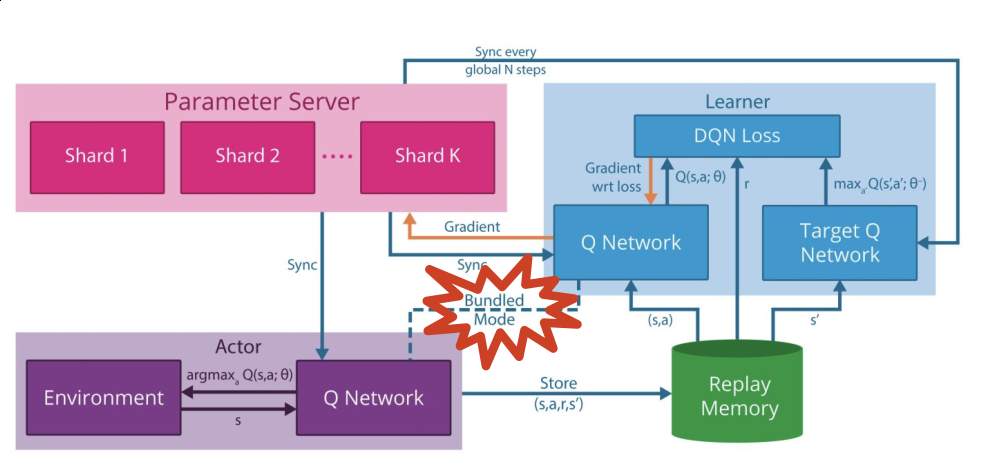
\includegraphics[width=0.8\textwidth]{figures/2020-07-13-142538_994x464_scrot.png}
    \end{center}
    Con esta arquitectura se mejora el resultado de casi todos los entornos de Atari, lo que
    lleva a pensar que escalar RL escogiendo las abstracciones adecuadas puede suponer un
    gran paso hacia adelante.
\item A3C (2016): es una gran mejora sobre GORILA. Una de sus características más
    sobresalientes es que se puede entrenar en una sola máquina. Esto permite evitar los
    cuellos de botella generados en las comunicaciones cuando se tienen varios componentes.
    También permite no usar un replay buffer.
\begin{center}
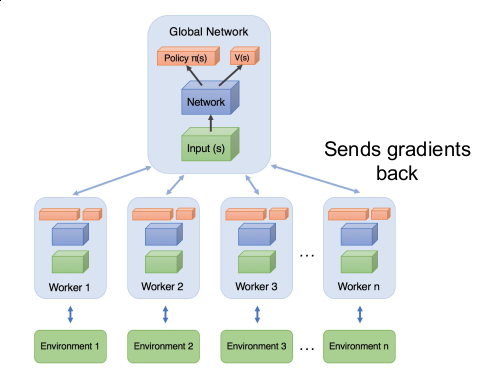
\includegraphics[width=0.5\textwidth]{figures/2020-07-13-143306_481x381_scrot.png}
\end{center}
    \item Importance Weighted Actor-Learner Architectures (IMPALA, 2018): se tienen varias
        copias de Learners y Actors. Los Actors tienen su propia copia de la red neuronal y
        actúan continuamente en sus entornos, generando una inmensa cantidad de datos. Por otro
        lado los Learners se encargan de distribuir la computación de la optimización. Como las
        redes que actúan no son las mismas que las que se están optimizando se usa un
        algoritmo de \textit{Importance Sampling} llamado \textit{V-tracing}. En la publicación
        muestran que este algoritmo consigue estabilizar el proceso de aprendizaje.
\begin{center}
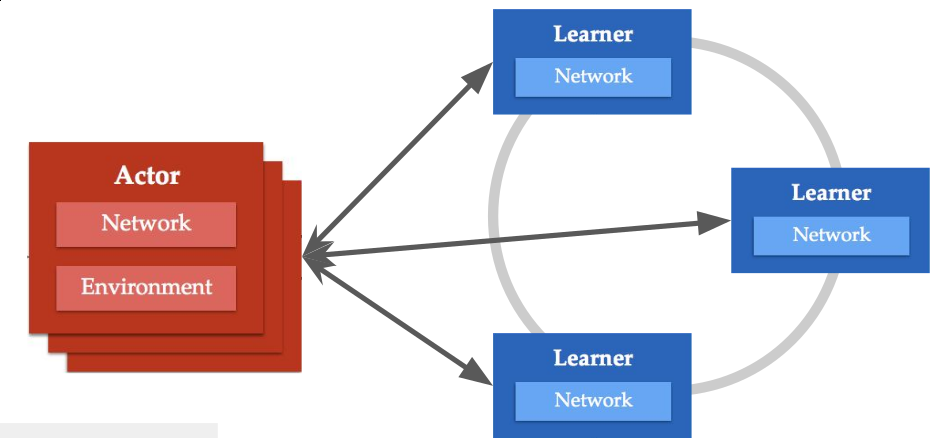
\includegraphics[width=0.6\textwidth]{figures/2020-07-13-143822_930x438_scrot.png}
\end{center}
    \item Ape-X/R2D2 (2018): da un paso atrás hacia GORILA y reaparece el replay buffer. Se
        tienen Actores corriendo asíncronamente y guardando las observaciones en el replay
        buffer. Otro proceso coge muestras del buffer y las usa para entrenar a la política.
        El buffer y el Learner son independientemente escalables. La novedad de esta
        arquitectura está en el buffer, que se ordena usando \textit{Distributed
        Prioritization}. Comparado con A3C y DQN escala extremadamente bien.
\begin{center}
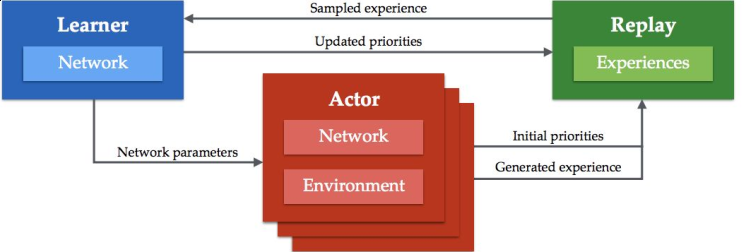
\includegraphics[width=0.8\textwidth]{figures/2020-07-13-150358_749x252_scrot.png}
\end{center}
    \item R2D3 (Ape-X con demostraciones, 2019): una arquitectura similar que permite el uso de
        datos de entrenamiento generados por humanos o un profesor.
        Se tienen dos buffers, el \textit{demo replay} y el \textit{agent replay}, de los
        cuales se muestrea con probabilidad $\rho$ y $1-\rho$ respectivamente.
\begin{center}
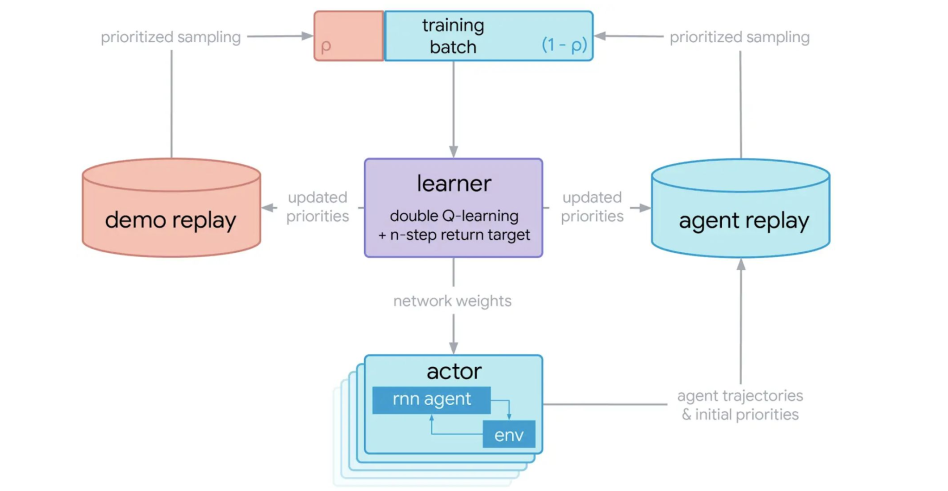
\includegraphics[width=0.6\textwidth]{figures/2020-07-13-150637_948x491_scrot.png}
\end{center}
\end{itemize}

\subsection{Otras arquitecturas distribuidas interesantes}%
\label{sub:otras_arquitecturas_distribuidas_interesantes}

\subsubsection{QT-Opt}%
\label{ssub:qt_opt}

Es una arquitectura que se conecta con el mundo real mediante robots. Consigue hacer un
bucle cerrado para entrenarlos en la tarea de la manipulación de objetos. 

\begin{center}
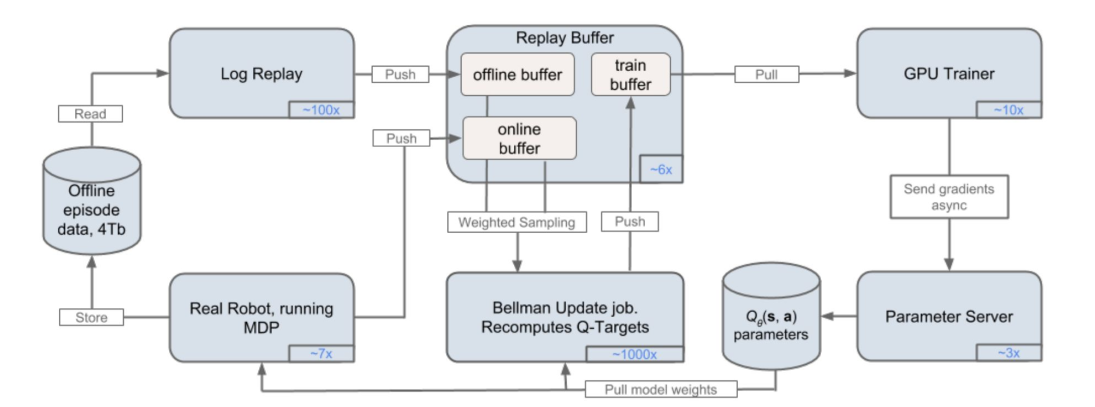
\includegraphics[width=0.8\textwidth]{figures/2020-07-13-172142_1095x407_scrot.png}
\end{center}

Abajo a la izquierda se tienen a los robots generando experiencia. Estos datas se meten en un
almacenamiento y posteriormente en un buffer. El replay buffer recibe experiencias
inmediatas y guardadas en el buffer.

\subsubsection{Estrategias de evolución}%
\label{ssub:estrategias_de_evolución}

Consisten en algoritmos de optimización altamente paralelizables. Cada agente tiene su copia
del entorno y de la red neuronal y cada red es ligeramente perturbada por un ruido y
produce una trayectoria.

\begin{algorithm}
    \caption{Estrategias de evolución paralelizables}
    \KwIn{Learning rate $\alpha$, desviación estándar del ruido $\sigma$, parámetros
    iniciales $\theta_0$}
    Inicializar $n$ trabajadores con semillas aleatorias conocidas y parámetros iniciales
    $\theta_0$\\
    \For{$t=1,2,3,\ldots$}{
    \For{cada trabajador $i=1,\ldots,n$}{
        Sacar una muestra $\epsilon\sim N(0,I)$\\
        Calcular las recompensas $F_i=F(\theta_t+\sigma\epsilon_i)$
    }
    Enviar todos los escalares  $F_i$ de cada trabajador a los demás trabajadores.\\
    \For{cada trabajador $i=1,\ldots,n$}{
        Reconstruir todas las perturbaciones $\epsilon_j$ para todo $j=1,\ldots,n$ usando las
        semillas aleatorias conocidas.\\
        $\theta_{t+1}\gets\theta_t \alpha \frac{1}{n\sigma}\sum_{j=1}^n
        F_j\epsilon_j$
    }
}
\end{algorithm}

\subsubsection{Más allá de RL: Entrenamiento basado en población}%
\label{ssub:más_allá_de_rl_entrenamiento_basado_en_población}

Es un método de búsqueda de hiperparámetros creado por DeepMind que comienza siendo como una
búsqueda aleatoria. Pero posteriormente en cada iteración los modelos que no se estén
comportando tan bien como el resto son modificados para mejorarlos.

Esto puede ayudar en mejorar los modelos existentes en un 5\% aproximadamente.

\section{RLlib: Abstractions for Distributed Reinforcement Learning (ICML 2018)}%
\label{sec:rllib_abstractions_for_distributed_reinforcement_learning_icml_2018_}

 Últimamente el hardware se está haciendo mucho más potente y barato, pero no todo el mundo
 tiene la infraestructura de software para hacer uso de todos estos beneficios. Para la creación
 de modelos existen múltiples librerías excelentes que ofrecen abstracciones como Tensorflow
 o PyTorch. Pero en el mundo de RL no existía una abstracción para la creación de algoritmos
 escalables.

 Si se mira a los algoritmos implementados hasta ahora, la mayoría de ellos usa MPI, Redis,
 Multiprocessing, Distributed TF, \ldots. En github existen aproximadamente 16000
 implementaciones de algoritmos de RL y no comparten la misma base de código.

 Los desafíos para la creación de una base de código reusable son:
 \begin{itemize}
     \item Un amplio rango de estrategias de ejecución físicas para un algoritmo.
\begin{center}
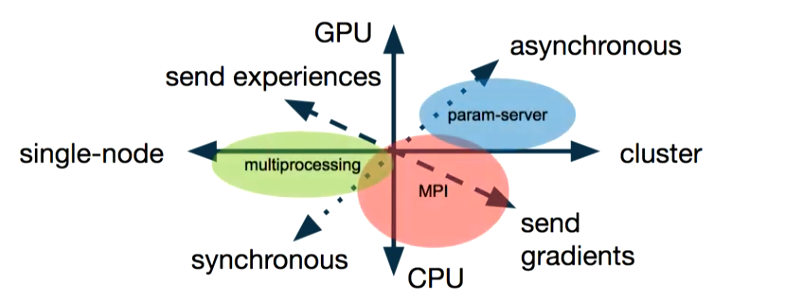
\includegraphics[width=0.5\textwidth]{figures/2020-07-13-180710_787x295_scrot.png}
\end{center}
     \item Las implementaciones están fuertemente acopladas a la librería usada para crear los
         modelos (PyTorch, Tensorflow, \ldots).
    \item Gran variedad de algoritmos con diferentes estructuras.
\end{itemize}

Con Ray se puede crear una instancia de clase en el cluster (\textit{statefull workers})
y después ir asignando pequeñas tareas a esos trabajadores. El desafío está en que mantenga
un alto rendimiento: 1e6+ tareas/s, ~200us por tarea.

Se pueden crear arquitecturas jerárquicas, en las que un trabajador tiene subtrabajadores y esos
tienen subsubtrabajadores.

\begin{center}
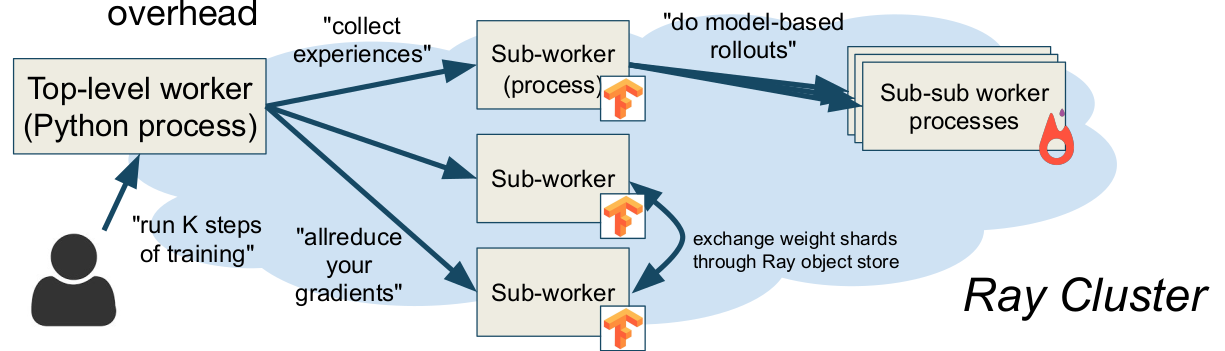
\includegraphics[width=0.8\textwidth]{figures/2020-07-13-185611_1225x351_scrot.png}
\end{center}

En resumen, RLlib está por encima de una simple colección de algoritmos. Las abstracciones
permiten implementar y escalar fácilmente nuevos algoritmos.

\begin{center}
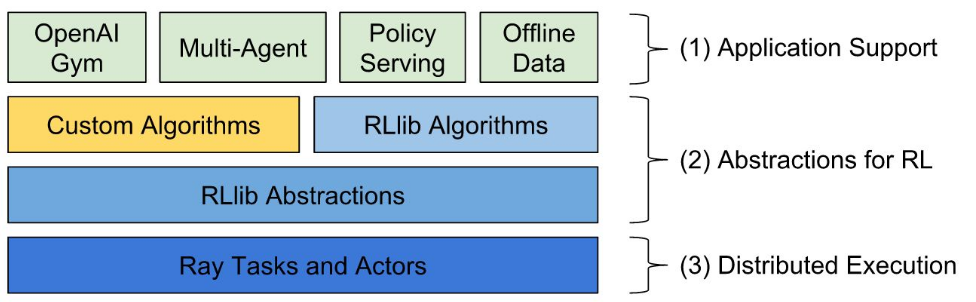
\includegraphics[width=0.8\textwidth]{figures/2020-07-13-185917_976x302_scrot.png}
\end{center}
   

